\chapter{Fisiología molecular vegetal y respuestas al estrés}\label{ch:b3:plant-molecular-physiology}

Una plántula de judía crecida en un armario a oscuras es una cosa
pálida y desgarbada: un tallo largo y blanco, un gancho en lo alto, dos
hojas amarillas plegadas. Llévesela a una ventana y en un día habrá
dejado de alargarse, habrá enderezado el gancho y habrá extendido y
vuelto verdes sus hojas ---otro organismo, a partir de los mismos
genes. No estaba esperando energía; estaba esperando información. Un
fotón rojo absorbido por una sola proteína le dice que ha alcanzado la
luz; la razón entre el rojo y el rojo lejano le dice si tiene encima la
hoja de un vecino; la duración de la noche le dice la estación; una
caída del potencial hídrico de sus raíces, un roce de viento, la
flagelina de una bacteria sobre su hoja ---cada cosa la detecta un
receptor, se convierte en una señal química y se responde con un cambio
en qué genes se expresan y qué células crecen. Una planta no puede huir
de su ambiente; ha de leerlo y remodelarse. Este capítulo trata de esa
lectura: los fotorreceptores, las \omterm{def:b3:endocrinology:hormone}{hormonas} y cómo actúan a escala
molecular, las respuestas a la sequía, la sal, el frío y el calor, y el
sistema inmunitario de dos capas que las plantas desarrollaron sin una
sola célula móvil.

\section{Leer la luz}

\begin{definition}[Fotorreceptores]\label{def:b3:plant-molecular-physiology:photoreceptors}
\index{fitocromo}\index{criptocromo}\index{fototropina}\index{fotomorfogénesis}\index{etiolación}
Las plantas perciben la luz con tres familias de proteínas, ninguna de
ellas clorofila. Los \emph{fitocromos} son dímeros con un pigmento
bilínico que la luz roja (\qty{660}{nm}) conmuta de la forma inactiva
\emph{Pr} a la activa \emph{Pfr}, y el rojo lejano (\qty{730}{nm})
devuelve; Pfr entra en el núcleo y marca para su degradación a una
familia de factores de transcripción, los PIF, lo que libera los genes
del desarrollo a la luz; en la oscuridad Pfr revierte despacio. Los
\emph{criptocromos} (azul, \qty{450}{nm}) son flavoproteínas
emparentadas con enzimas de reparación del ADN, y gobiernan la
desetiolación, el reloj y la floración; las \emph{fototropinas} (azul)
son cinasas de membrana que dirigen la curvatura hacia la luz, la
apertura de los estomas y el movimiento de los cloroplastos. Una
plántula a oscuras está \emph{etiolada} ---hipocótilo largo,
cotiledones cerrados, sin clorofila, con todos los recursos gastados en
alcanzar la superficie---; la luz la conmuta a la
\emph{fotomorfogénesis}, y el interruptor lo accionan Pfr y el
criptocromo al inactivar un único complejo represor (COP1) que en la
oscuridad destruye los factores de transcripción del programa de luz.
La luz se lee, pues, dos veces: como energía, por el cloroplasto, y
como señal, por receptores sensibles a flujos de fotones un millón de
veces menores.
\end{definition}

\begin{proposition}[El fotoequilibrio del fitocromo]\label{prop:b3:plant-molecular-physiology:photoequilibrium}
\index{fotoequilibrio}\index{razón rojo:rojo lejano}\index{evitación de la sombra}
Bajo luz continua, Pr y Pfr se interconvierten hasta que las dos
velocidades de fotoconversión se equilibran: con $k_{1}$ la velocidad
de Pr $\to$ Pfr (proporcional al flujo rojo) y $k_{2}$ la de Pfr $\to$
Pr (proporcional al flujo de rojo lejano, más algo del rojo, que Pfr
también absorbe), la fracción de forma activa es
\[
\varphi = \frac{[\text{Pfr}]}{[\text{Pfr}] + [\text{Pr}]} = \frac{k_{1}}{k_{1} + k_{2}},
\]
independiente del flujo total y fijada solo por la \emph{\omterm{prop:b3:plant-molecular-physiology:photoequilibrium}{razón
rojo:rojo lejano}} $\zeta$ de la luz. El rojo puro da
$\varphi \approx 0.87$ (Pfr absorbe también algo de rojo); el rojo
lejano puro, $0.03$; la luz del día a cielo abierto, $\zeta \approx
1.15$, da alrededor de $0.55$, y la luz bajo una cubierta de hojas,
cuya clorofila ha retirado el rojo y ha dejado pasar el rojo lejano,
tiene $\zeta \approx 0.2$ y $\varphi \approx 0.2$. Una planta lee su
$\varphi$ como la presencia de vecinos: un valor bajo dispara el
síndrome de \emph{\omterm{prop:b3:plant-molecular-physiology:photoequilibrium}{evitación de la sombra}} ---tallos alargados, hojas
levantadas, floración temprana, menos ramificación--- a través de los
PIF que Pfr ya no destruye. La plantación densa de un agricultor es una
carrera de plantas que huyen de la sombra; los trigos enanos de la
Revolución Verde, insensibles a la señal, pusieron en el grano el
crecimiento ahorrado.
\end{proposition}
\begin{proof}
$\mathrm{d}[\text{Pfr}]/\mathrm{d}t = k_{1}[\text{Pr}] - k_{2}[\text{Pfr}]$
con $[\text{Pr}] + [\text{Pfr}] = P$ fijo da, en estado estacionario,
$k_{1}(P - [\text{Pfr}]) = k_{2}[\text{Pfr}]$, de donde $\varphi = k_{1}/
(k_{1} + k_{2})$. Ambas velocidades son proporcionales al flujo
incidente, de modo que escalar la luz escala las dos y deja $\varphi$
sin cambio; solo importa la composición espectral. El estado
estacionario se alcanza con una velocidad $k_{1} + k_{2}$ ---segundos a
pleno sol, minutos al atardecer--- y la reversión en la oscuridad de
Pfr, con una semivida de horas, fija lo que queda por la noche.
\end{proof}

\begin{omfigure}
\begin{tikzpicture}[every node/.style={font=\scriptsize}, >=stealth]
  \node[draw, very thick, omDef, fill=omDef!15, rounded corners, minimum width=1.6cm, minimum height=0.9cm] (pr) at (0,0) {Pr (inactivo)};
  \node[draw, very thick, omThm, fill=omThm!15, rounded corners, minimum width=1.6cm, minimum height=0.9cm] (pfr) at (4.2,0) {Pfr (activo)};
  \draw[->, very thick, red!70!black] (pr.north east) to[bend left=25] node[above] {rojo, \qty{660}{nm}} (pfr.north west);
  \draw[->, very thick, red!40!black] (pfr.south west) to[bend left=25] node[below] {rojo lejano, \qty{730}{nm}} (pr.south east);
  \draw[->, thick, gray] (pfr.south) ++(0.5,-0.15) to[bend left=40] node[right, font=\tiny, gray] {reversión en la oscuridad, horas} ++(-0.3,-0.9);
  \draw[->, thick] (pfr.east) -- ++(1.0,0) node[right, align=left] {hacia el núcleo:\\PIF degradados, COP1 apagado;\\programa de luz encendido};
  \begin{scope}[shift={(0,-4.6)}]
  \begin{axis}[
    width=0.55\linewidth, height=4.6cm,
    axis x line=bottom, axis y line=left,
    xmin=0, xmax=2.5, ymin=0, ymax=1,
    xlabel={razón rojo:rojo lejano $\zeta$}, ylabel={$\varphi = $ fracción de Pfr},
    xlabel style={font=\scriptsize, at={(axis description cs:0.5,-0.15)}, anchor=north}, ylabel style={font=\scriptsize},
    tick label style={font=\scriptsize}, xtick={0.2,0.5,1.15,2}, xticklabels={0.2,0.5,1.15,2}, ytick={0.2,0.55,0.87},
    clip=false,
  ]
  \addplot[very thick, omDef, domain=0:2.5, samples=80] {0.87*x/(x+0.6)};
  \draw[dashed, gray] (axis cs:0.2,0) -- (axis cs:0.2,0.22) -- (axis cs:0,0.22);
  \draw[dashed, gray] (axis cs:1.15,0) -- (axis cs:1.15,0.57) -- (axis cs:0,0.57);
  \node[font=\tiny, anchor=west, align=left] at (axis cs:0.25,0.12) {bajo una cubierta:\\evitación de la sombra};
  \node[font=\tiny, anchor=south west] at (axis cs:1.2,0.62) {luz del día abierta};
  \node[font=\tiny, anchor=north west, omDef, align=left] at (axis cs:1.6,0.45) {un ajuste empírico,\\$\varphi \approx 0.87\,\zeta/(\zeta + 0.6)$};
  \end{axis}
  \end{scope}
\end{tikzpicture}

{\small El interruptor del \omterm{def:b3:plant-molecular-physiology:photoreceptors}{fitocromo}. La luz roja fabrica la forma
activa, el rojo lejano la deshace y la oscuridad la revierte despacio;
la fracción estacionaria de forma activa depende del equilibrio de
colores de la luz y no de su brillo, que es como una plántula sabe que
tiene una hoja encima.}
\end{omfigure}

\begin{proof}[Evidencia]
Borthwick, Hendricks y sus colaboradores (1952) dieron destellos breves
a semillas de lechuga: el rojo las hacía germinar, el rojo lejano dado
después lo cancelaba, el rojo de nuevo lo restauraba, y así a lo largo
de una docena de alternancias ---decidía el último destello, la firma
de un pigmento reversible, que después extrajeron (1959) como una
proteína azul que cambiaba su espectro de absorción con el rojo y el
rojo lejano. Más tarde se demostró que todo el programa de la plántula
crecida a oscuras pende de un solo represor: los mutantes sin COP1 se
desarrollan en oscuridad total como si estuvieran a la luz, cortos y
listos para verdear, y los mutantes deficientes en \omterm{def:b3:plant-molecular-physiology:photoreceptors}{fitocromo} y en
\omterm{def:b3:plant-molecular-physiology:photoreceptors}{criptocromo} siguen etiolados a la luz.
\end{proof}

\begin{omfigure}
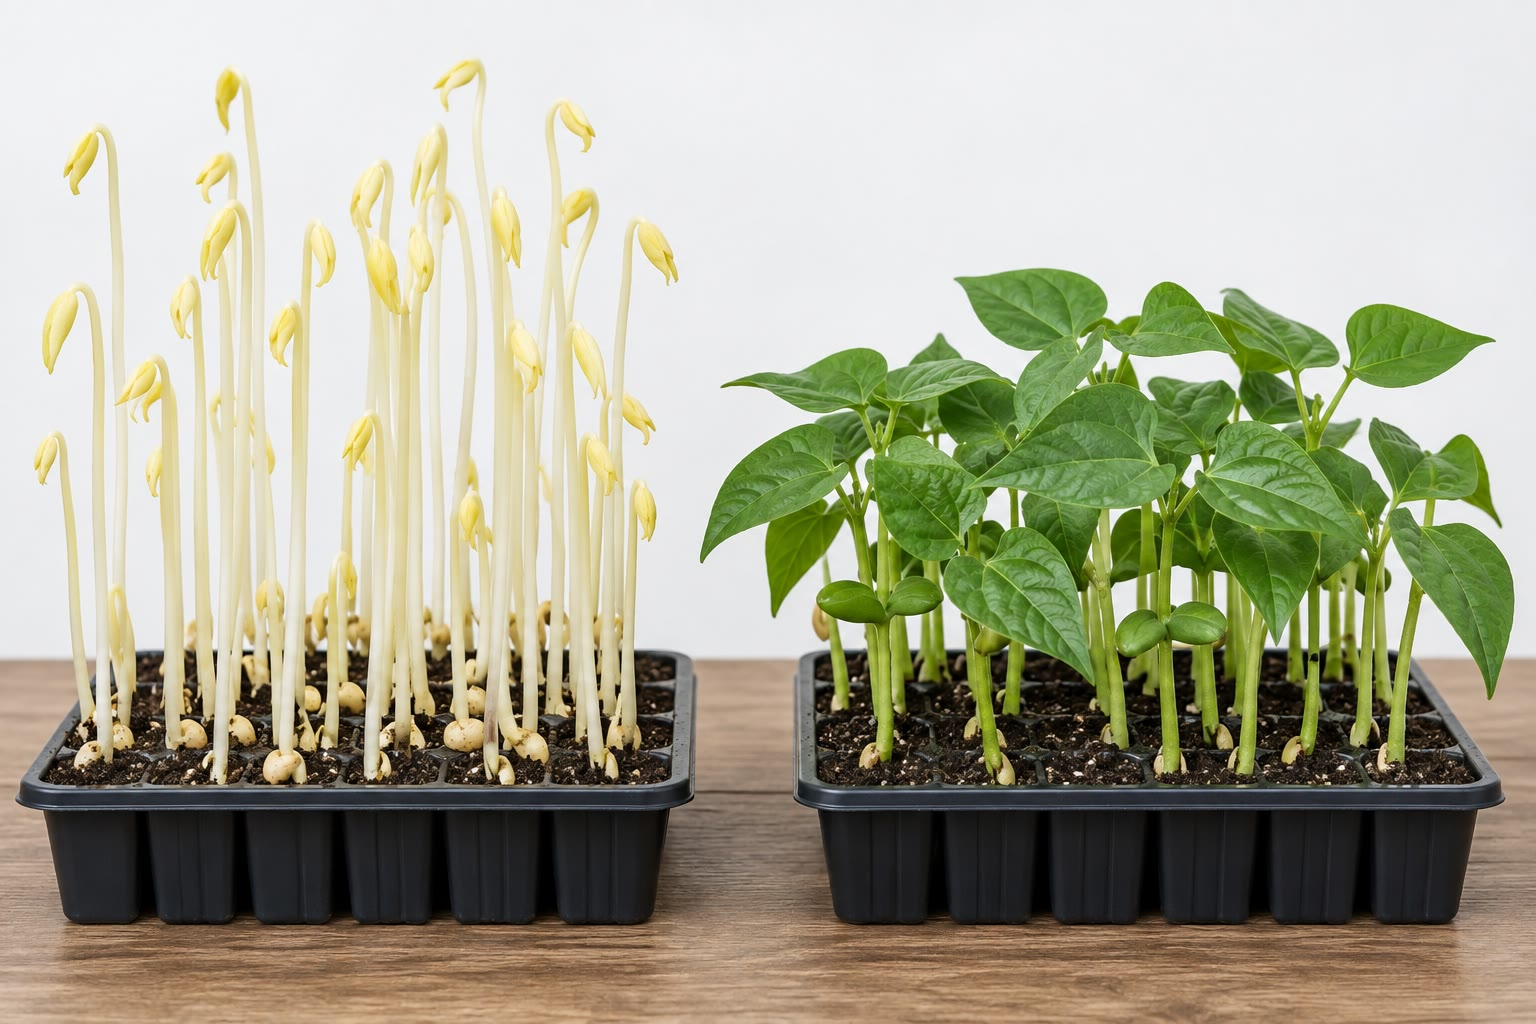
\includegraphics[width=0.56\linewidth]{images/book5/ai/b5-22-etiolated-seedlings.jpg}

{\small Plántulas crecidas en la oscuridad y a la luz: el mismo genoma,
dos programas de desarrollo, y la diferencia es un solo fotón rojo
absorbido por el \omterm{def:b3:plant-molecular-physiology:photoreceptors}{fitocromo}.}
\end{omfigure}

\section{Las hormonas a escala molecular}

\begin{definition}[Las hormonas vegetales y sus receptores]\label{def:b3:plant-molecular-physiology:hormones}
\index{auxina}\index{TIR1}\index{giberelina}\index{DELLA}\index{ácido abscísico}\index{etileno}\index{citoquinina}\index{brasinoesteroide}
El volumen del Año~1 describió qué hacen las \omterm{def:b3:endocrinology:hormone}{hormonas} vegetales; aquí
va cómo se las oye. Varias actúan por \emph{destrucción regulada}. La
\emph{auxina} (ácido indol-3-acético) se une a la proteína F-box
\emph{TIR1} y la pega a los represores Aux/IAA, que quedan entonces
ubiquitinados y son destruidos por el proteasoma: los genes de
respuesta a la auxina que reprimían se encienden en minutos ---la
\omterm{def:b3:endocrinology:hormone}{hormona} es un pegamento molecular, y el receptor forma parte de la
maquinaria de degradación. La \emph{giberelina} hace lo mismo con los
represores \emph{DELLA} del crecimiento, a través de su receptor GID1:
los trigos y arroces enanos de la Revolución Verde llevan proteínas
DELLA que no pueden destruirse y por eso siguen siendo bajos por mucha
giberelina que fabriquen. El \emph{jasmonato} sigue la misma lógica con
los represores JAZ. El \emph{ácido abscísico} (ABA), la \omterm{def:b3:endocrinology:hormone}{hormona} de la
sequía y de la latencia, se une a los receptores PYR/PYL, que inhiben
entonces una fosfatasa (PP2C) y liberan una cinasa (SnRK2) que fosforila
canales iónicos y factores de transcripción ---una doble negación que
vuelve empinada la respuesta. El \emph{etileno}, un gas, se une a
receptores con cobre de la membrana del retículo que, en su ausencia,
reprimen activamente la respuesta; al unirse los apaga, y se encienden
los genes de la maduración, la \omterm{def:b3:cell-cycle-apoptosis:other}{senescencia} y el estrés. Las
\emph{citoquininas} actúan a través de receptores de histidina-cinasa
como los sistemas bacterianos de dos componentes; los
\emph{brasinoesteroides}, los esteroides de la planta, a través de una
cinasa receptora de superficie y no de un \omterm{def:b3:endocrinology:hormone}{receptor nuclear} ---las
únicas \omterm{def:b3:endocrinology:hormone}{hormonas esteroideas} que en parte alguna se oyen en la
superficie celular. Las plantas no tienen glándulas: cada \omterm{def:b3:endocrinology:hormone}{hormona} se
fabrica donde hace falta, o la mueven transportadores específicos, y su
concentración la fijan localmente la síntesis, la conjugación y la
destrucción.
\end{definition}

\begin{theorem}[Transporte polar quimiosmótico de la auxina]\label{thm:b3:plant-molecular-physiology:auxin}
\index{transporte polar de auxina}\index{proteínas PIN}\index{atrapamiento aniónico}
El ácido indol-3-acético es un ácido débil, $\mathrm{p}K_{a} = 4.75$.
En el espacio de la pared celular, a pH~$5.5$, una fracción
apreciable es el IAAH neutro, que difunde a través de la membrana; en
el citosol, a pH~$7.2$, casi todo es el anión IAA$^{-}$, que no puede
salir por difusión. En el equilibrio de la forma neutra a través de la
membrana, la razón entre la \omterm{def:b3:plant-molecular-physiology:hormones}{auxina} total de dentro y la de fuera es
\[
\frac{[\text{IAA}]_{\text{int}}}{[\text{IAA}]_{\text{ext}}}
= \frac{1 + 10^{\,\mathrm{pH}_{\text{int}} - \mathrm{p}K_{a}}}{1 + 10^{\,\mathrm{pH}_{\text{ext}} - \mathrm{p}K_{a}}}
\approx \frac{283}{6.6} \approx 43 :
\]
la célula atrapa la \omterm{def:b3:plant-molecular-physiology:hormones}{auxina} cuarenta veces. Solo puede salir por los
transportadores de expulsión \emph{PIN}, y como cada célula coloca sus
PIN en una sola cara ---la basal, en el tallo---, la \omterm{def:b3:plant-molecular-physiology:hormones}{auxina} captada por
todas partes sale por abajo, entra en la célula siguiente, y así
sucesivamente: una columna de células con la misma polaridad es una
cinta transportadora que mueve la \omterm{def:b3:plant-molecular-physiology:hormones}{auxina} a alrededor de \qty{1}{cm/h}
desde el ápice del brote hasta la raíz, y reorientar los PIN redirige
la corriente, que es como un lado sombreado de un tallo llega a
contener más \omterm{def:b3:plant-molecular-physiology:hormones}{auxina} y a crecer más deprisa.
\end{theorem}
\begin{proof}
Henderson--Hasselbalch: $[\text{IAA}^{-}]/[\text{IAAH}] = 10^{\,\mathrm{pH}
- \mathrm{p}K_{a}}$, de modo que el total $= [\text{IAAH}](1 + 10^{\,\mathrm{pH} -
\mathrm{p}K_{a}})$. La forma neutra se equilibra, $[\text{IAAH}]_{\text{int}}
= [\text{IAAH}]_{\text{ext}}$; dividir los totales da la razón,
$(1 + 10^{2.45})/(1 + 10^{0.75}) = 283/6.6$. Con los PIN en una sola
cara, la única salida del anión es direccional; una columna de $n$
células se pasa el flujo, y la velocidad medida, un orden de magnitud
por encima de la difusión a estas distancias, es la de una expulsión
mediada por transportadores en cada límite celular. La hipótesis de
Cholodny--Went (años veinte), según la cual la curvatura sigue a una
redistribución lateral de \omterm{def:b3:plant-molecular-physiology:hormones}{auxina}, se confirmó por medida directa en
coleóptilos de avena y por imagen de la reubicación de los PIN en
raíces de \emph{Arabidopsis} tumbadas de lado (años dos mil).
\end{proof}

\begin{omfigure}
\begin{tikzpicture}[every node/.style={font=\scriptsize}, >=stealth]
  % three cells in a column
  \foreach \y in {0,-2.2,-4.4} {
    \draw[thick, omDef, fill=omDef!8] (0,\y) rectangle (3.2,\y-1.9);
    \draw[very thick, omThm] (0.6,\y-1.9) -- (2.6,\y-1.9);
    \node[right, font=\tiny] at (3.3,\y-0.4) {citosol pH 7,2};
    \node[right, font=\tiny] at (3.3,\y-0.8) {IAA$^{-}$ atrapado};
    \draw[->, thick, omDef!70!black] (-0.6,\y-0.6) -- (0.4,\y-0.6); \node[left, font=\tiny] at (-0.6,\y-0.6) {entra IAAH};
    \draw[->, thick, omDef!70!black] (3.8,\y-1.3) -- (2.8,\y-1.3);
    \draw[->, very thick, omThm] (1.6,\y-1.5) -- (1.6,\y-2.35);
  }
  \node[left, align=right, font=\tiny] at (-0.6,-1.4) {pared a pH 5,5:\\\qty{15}{\%} IAAH,\\\qty{85}{\%} IAA$^{-}$};
  \node[omThm, right, font=\tiny] at (3.3,-2.05) {transportadores de expulsión PIN, solo en la cara basal};
  \node[above] at (1.6,0.1) {ápice del brote: fuente de auxina};
  \node[below] at (1.6,-6.8) {hacia la raíz, \qty{1}{cm/h}};
  \node[right, align=left] at (5.4,-3.6) {dentro : fuera $\approx 43 : 1$\\(atrapamiento del anión)\\[3pt]salida solo por los PIN,\\de modo que la columna es una cinta;\\muévanse los PIN a una cara lateral\\y la corriente gira};
\end{tikzpicture}

{\small El modelo quimiosmótico del \omterm{thm:b3:plant-molecular-physiology:auxin}{transporte polar de auxina}. El
ácido entra por cualquier cara como molécula neutra, queda atrapado
como anión al pH del citosol y sale solo por transportadores que la
célula ha colocado en una cara ---de modo que una fila de células pasa
la \omterm{def:b3:plant-molecular-physiology:hormones}{auxina} en un solo sentido.}
\end{omfigure}

\begin{example}[Gravitropismo y fototropismo]\label{ex:b3:plant-molecular-physiology:tropism}
Túmbese de lado una plántula. En la cofia de la raíz, unos plastos
densos llenos de almidón se posan en minutos sobre el nuevo lado
inferior de las células de la columela; los transportadores PIN3 de
esas células se reubican en la cara inferior; la \omterm{def:b3:plant-molecular-physiology:hormones}{auxina} fluye
preferentemente por el flanco inferior de la raíz, donde, por encima
del óptimo de las células radiculares, \emph{inhibe} la elongación, y
la raíz se curva hacia abajo. En el brote, el mismo flujo lateral hacia
el lado inferior \emph{favorece} la elongación (el óptimo de las
células del brote es más alto), y el brote se curva hacia arriba.
Fototropismo: la \omterm{def:b3:plant-molecular-physiology:photoreceptors}{fototropina} del lado iluminado de un brote altera la
colocación de los PIN de modo que la \omterm{def:b3:plant-molecular-physiology:hormones}{auxina} se acumula en el lado
sombreado, que crece más deprisa y curva el brote hacia la luz. Ambos
movimientos son lentos ---horas--- porque son crecimiento y no
movimiento, y ambos son irreversibles en el tejido que ha crecido.
Darwin (1880) mostró que el ápice de una plántula de gramínea percibe
la luz y que la región de debajo se curva; Went (1928) recogió la
influencia en un bloque de agar colocado sobre un ápice cortado y
mostró que un bloque puesto de forma asimétrica sobre un brote
decapitado lo hacía curvarse: la influencia era una sustancia
difusible, a la que se llamó después \omterm{def:b3:plant-molecular-physiology:hormones}{auxina}.
\end{example}

\section{Agua, sal, frío y calor}

\begin{definition}[El estrés abiótico]\label{def:b3:plant-molecular-physiology:abiotic}
\index{estrés hídrico}\index{ajuste osmótico}\index{estrés salino}\index{aclimatación al frío}\index{proteínas de choque térmico}
Una planta no puede escapar, así que se endurece. La \emph{sequía}: la
caída del potencial hídrico en las raíces dispara la síntesis de ABA;
el ABA cierra los estomas en minutos y, a lo largo de días, enciende
genes para el \emph{ajuste osmótico} (se acumulan prolina, azúcares y
otros solutos compatibles, que bajan el potencial hídrico de la célula
para que siga atrayendo agua), para dehidrinas que protegen las
proteínas, y para una superficie foliar menor y una raíz más profunda.
La \emph{sal} es sequía más veneno: el sodio entra por los canales de
potasio y compite con el potasio; las plantas tolerantes lo devuelven
al exterior de las raíces (la vía SOS), lo meten en vacuolas
(intercambiadores NHX) o lo excretan por glándulas foliares, y su
extremo \emph{halófito} vive en agua de mar. El \emph{frío}: el
enfriamiento rigidiza las membranas y frena las enzimas; la congelación
extrae agua de las células hacia el hielo extracelular y las deseca. La
\emph{aclimatación al frío} ---una semana de días frescos--- induce los
factores de transcripción CBF, que encienden cientos de genes de
lípidos que fluidifican la membrana, azúcares, proteínas anticongelantes
y dehidrinas, y un centeno de invierno que moriría a
\qty{-5}{\celsius} en agosto sobrevive a \qty{-30}{\celsius} en enero.
El \emph{calor} desnaturaliza las proteínas; a los pocos minutos de una
subida, un factor de choque térmico libera \emph{proteínas de choque
térmico}, \omterm{def:b3:structural-biology:chaperones}{chaperonas} que las repliegan o las eliminan, de las mismas
familias que en todo organismo. La \emph{inundación} priva de oxígeno a
las raíces; el arroz fabrica canales de aire (aerénquima) y se alarga
para mantener las hojas por encima del agua, siendo el \omterm{def:b3:plant-molecular-physiology:hormones}{etileno} la señal
que se acumula cuando no puede escapar al agua. Muchos de estos
programas se solapan ---el ABA, las especies reactivas del oxígeno y
los picos de calcio son segundos mensajeros compartidos---, y una
planta aclimatada a un estrés suele quedar en parte protegida frente a
otro.
\end{definition}

\begin{proposition}[El estoma como válvula]\label{prop:b3:plant-molecular-physiology:stomata}
\index{estoma}\index{célula oclusiva}\index{conductancia estomática}\index{eficiencia en el uso del agua}
Un par de \emph{\omterm{prop:b3:plant-molecular-physiology:stomata}{células oclusivas}} delimita cada poro estomático; el
poro se abre cuando captan potasio y aniones (y fabrican azúcar), se
hinchan y se arquean separándose, y se cierra cuando los pierden. La
luz azul (\omterm{def:b3:plant-molecular-physiology:photoreceptors}{fototropinas}), el CO$_{2}$ bajo y la humedad lo abren; la
oscuridad, el CO$_{2}$ alto, la sequía y el ABA lo cierran. La ruta del
ABA: receptor $\to$ fosfatasa inhibida $\to$ cinasa activa $\to$
canales de aniones (SLAC1) abiertos $\to$ la membrana se despolariza
$\to$ el potasio sale por canales de salida $\to$ el agua lo sigue
$\to$ el poro se cierra, en diez minutos. El poro es donde se hace el
intercambio central de la planta: el CO$_{2}$ difunde hacia dentro y el
vapor de agua hacia fuera por el mismo agujero, y como el gradiente de
vapor (una hoja al \qty{100}{\%} de humedad por dentro frente a un aire
al \qty{50}{\%}) es cincuenta veces más empinado que el gradiente de
CO$_{2}$ (\qty{400}{ppm} fuera, \qty{250}{} dentro), una hoja pierde
varios cientos de moléculas de agua por cada molécula de carbono que
fija. La \emph{\omterm{prop:b3:plant-molecular-physiology:stomata}{conductancia estomática}} $g_{s}$ fija ambos flujos: la
transpiración $E = g_{s}\,\Delta w$ y la asimilación
$A = (g_{s}/1.6)\,\Delta c$ (el CO$_{2}$, más pesado, difunde $1.6$
veces más despacio), de modo que la \emph{\omterm{prop:b3:plant-molecular-physiology:stomata}{eficiencia en el uso del
agua}} $A/E = \Delta c/(1.6\,\Delta w)$ depende de los gradientes y no
de cuánto se abra el poro; cerrar el poro baja los dos flujos a la vez,
y elevar el CO$_{2}$ interno (las plantas C$_{4}$, que lo concentran) o
abrir solo de noche (las plantas CAM, en aire fresco y húmedo) es como
mejoran la razón las plantas del desierto.
\end{proposition}
\begin{proof}
La ley de Fick a través del poro para cada gas, con la misma
conductancia geométrica escalada por la razón de los coeficientes de
difusión $D_{\mathrm{H_2O}}/D_{\mathrm{CO_2}} = 1.6$; dividir los dos
flujos cancela $g_{s}$. Números: $\Delta w \approx \qty{15}{mmol/mol}$
de aire a \qty{25}{\celsius} y \qty{50}{\%} de humedad, $\Delta c \approx
\qty{150}{\micro mol/mol}$: $A/E = 150/(1.6\times\num{15000}) = 1/160$
---$160$ moléculas de agua por CO$_{2}$ en esas condiciones suaves, y
$500$ en aire seco. La secuencia de acción del ABA se estableció con
protoplastos de \omterm{prop:b3:plant-molecular-physiology:stomata}{células oclusivas} bajo pinza de membrana, con la
corriente aniónica apareciendo en menos de un minuto tras el ABA y el
mutante sin SLAC1 incapaz de cerrar.
\end{proof}

\begin{omfigure}
\begin{tikzpicture}[every node/.style={font=\scriptsize}, >=stealth]
  % pore with two guard cells
  \begin{scope}[shift={(0,0)}]
    \fill[omProp!30] (0,0) ellipse (1.4 and 0.9);
    \fill[white] (0,0) ellipse (0.5 and 0.6);
    \draw[thick, omProp!80!black] (0,0) ellipse (1.4 and 0.9); \draw[thick, omProp!80!black] (0,0) ellipse (0.5 and 0.6);
    \node[below, font=\tiny] at (0,-1.0) {abierto: entran K$^{+}$, Cl$^{-}$ y malato, turgente};
    \draw[->, thick, omDef] (0,0.3) -- (0,1.5) node[above, font=\tiny] {sale H$_2$O, $E = g_{s}\Delta w$};
    \draw[->, thick, omThm] (0,1.5) ++(-1.0,0) -- ++(0,-1.2); \node[left, font=\tiny, omThm] at (-1.1,1.0) {entra CO$_2$, $A = g_{s}\Delta c/1.6$};
  \end{scope}
  \begin{scope}[shift={(4.2,0)}]
    \fill[omProp!30] (0,0) ellipse (1.2 and 0.75);
    \draw[thick, omProp!80!black] (0,0) ellipse (1.2 and 0.75); \draw[very thick, omProp!80!black] (0,-0.5) -- (0,0.5);
    \node[below, font=\tiny] at (0,-0.9) {cerrado: iones perdidos, flácido};
  \end{scope}
  \draw[->, thick] (1.6,0) -- (2.8,0) node[midway, above, font=\tiny] {ABA, oscuridad,};
  \node[font=\tiny] at (2.2,-0.25) {CO$_2$ alto};
  % ABA pathway chain
  \begin{scope}[shift={(7.0,1.7)}]
    \node[draw, rounded corners, fill=omDef!20, align=center, font=\tiny] (a) at (0,0) {el ABA se une\\a PYR/PYL};
    \node[draw, rounded corners, fill=omThm!15, align=center, font=\tiny] (b) at (0,-0.9) {fosfatasa PP2C\\inhibida};
    \node[draw, rounded corners, fill=omMeth!25, align=center, font=\tiny] (c) at (0,-1.8) {cinasa SnRK2\\activa};
    \node[draw, rounded corners, fill=omProp!25, align=center, font=\tiny] (d) at (0,-2.7) {canal aniónico SLAC1\\abierto: despolarización};
    \node[draw, rounded corners, fill=omProp!25, align=center, font=\tiny] (e) at (0,-3.6) {sale K$^{+}$, sale agua,\\el poro se cierra en \qty{10}{min}};
    \draw[-|, thick] (a) -- (b); \draw[-|, thick] (b) -- (c); \draw[->, thick] (c) -- (d); \draw[->, thick] (d) -- (e);
    \node[right, font=\tiny, align=left] at (1.5,-0.9) {dos inhibiciones\\en serie:\\un interruptor brusco};
  \end{scope}
\end{tikzpicture}

{\small El estoma y la señal que lo cierra. El agua y el dióxido de
carbono comparten el poro, de modo que la planta cambia el uno por el
otro a un ritmo que fijan los dos gradientes; la \omterm{def:b3:endocrinology:hormone}{hormona} de la sequía
cierra la válvula mediante una cadena de dos inhibiciones, lo que
vuelve la respuesta parecida a un interruptor.}
\end{omfigure}

\begin{omfigure}
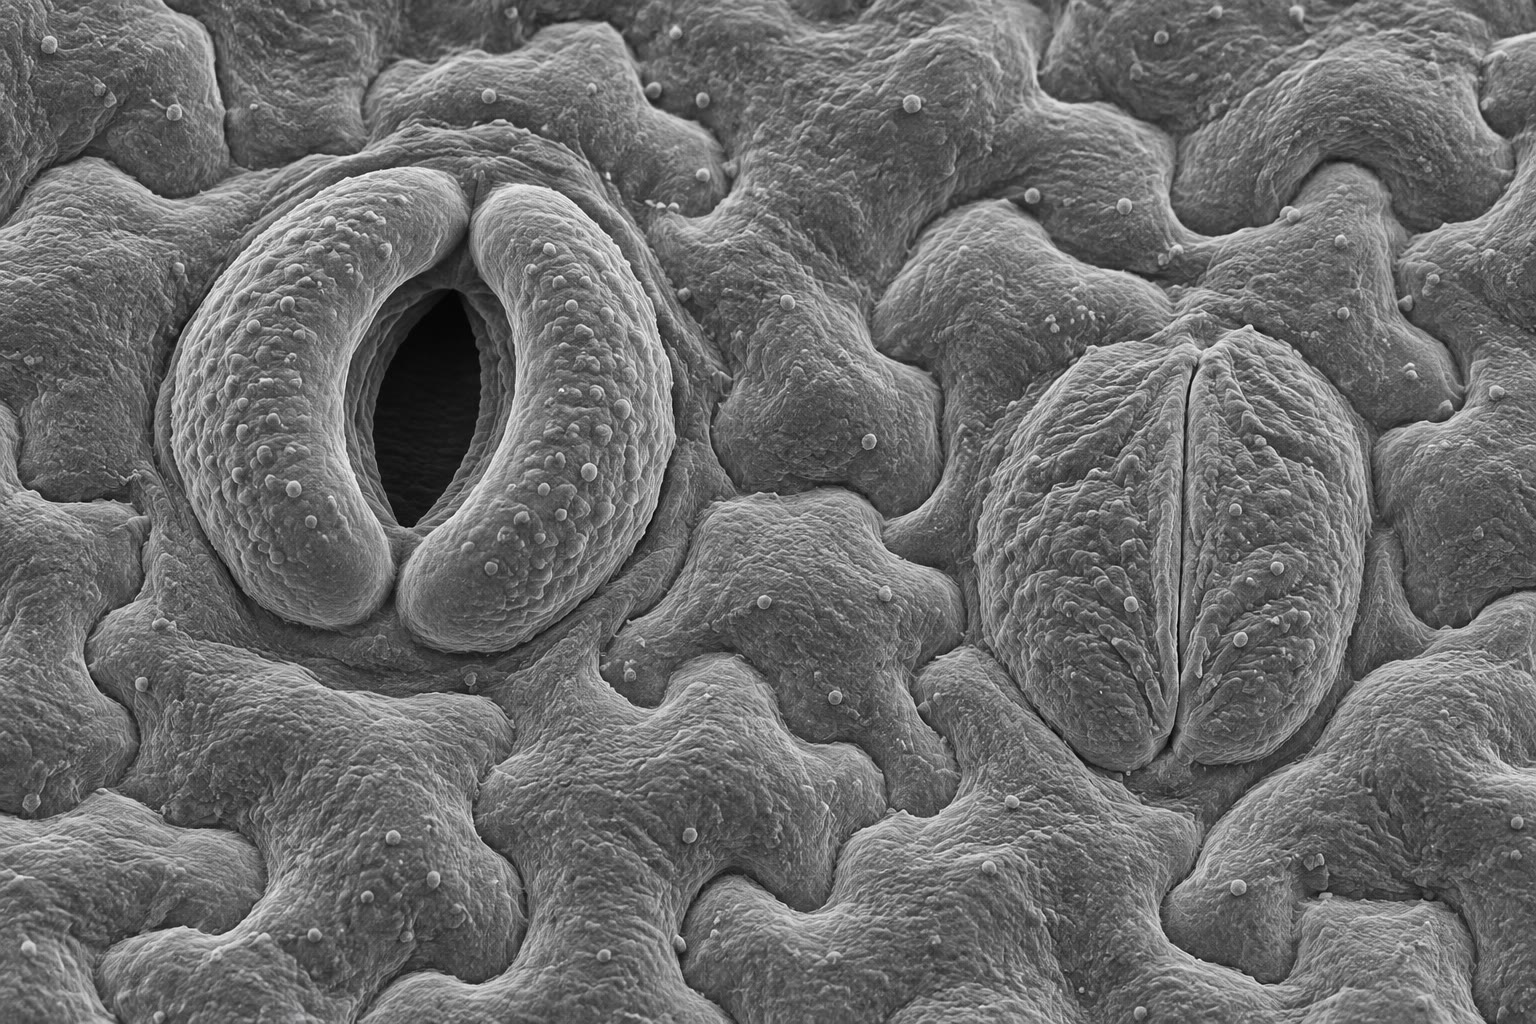
\includegraphics[width=0.46\linewidth]{images/book5/ai/b5-22-stomata-sem.jpg}\hspace{0.04\linewidth}
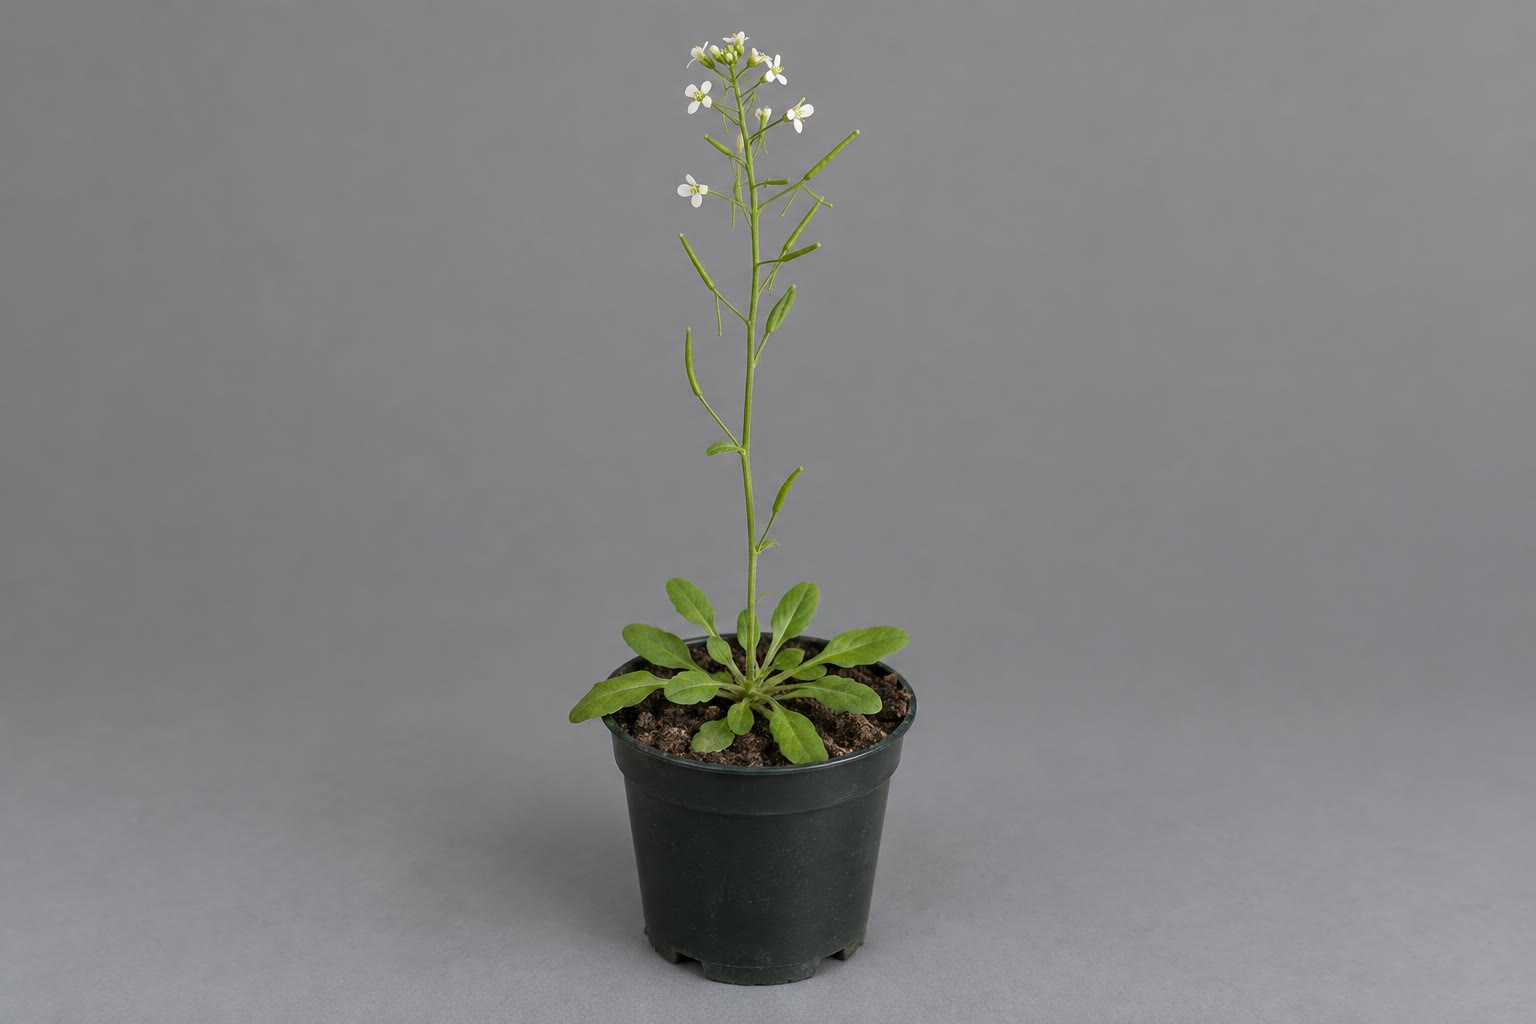
\includegraphics[width=0.46\linewidth]{images/book5/ai/b5-22-arabidopsis.jpg}

{\small Izquierda: estomas en la superficie de una hoja, cada poro
entre sus dos \omterm{prop:b3:plant-molecular-physiology:stomata}{células oclusivas}, unos abiertos y otros cerrados.
Derecha: \emph{Arabidopsis thaliana}, una mala hierba de cuneta con un
genoma pequeño, una generación de seis semanas y cien mil líneas
mutantes, en la que se hallaron casi todas las moléculas de este
capítulo.}
\end{omfigure}

\section{Inmunidad sin células inmunitarias}

\begin{definition}[Las dos capas de la inmunidad vegetal]\label{def:b3:plant-molecular-physiology:immunity}
\index{inmunidad desencadenada por patrones}\index{inmunidad desencadenada por efectores}\index{receptor NLR}\index{respuesta hipersensible}\index{resistencia sistémica adquirida}\index{ácido salicílico}\index{ácido jasmónico}
Toda célula vegetal es su propia célula inmunitaria. La primera capa,
la \emph{inmunidad desencadenada por patrones} (PTI), emplea cinasas
receptoras de superficie que reconocen moléculas comunes a clases
enteras de microbios ---FLS2 une un trozo de veintidós aminoácidos de
la flagelina bacteriana, y otras unen fragmentos de quitina de las
paredes fúngicas--- y en minutos lanza una entrada de calcio, una
explosión de oxígeno reactivo, cascadas de cinasas, el cierre de los
estomas, el engrosamiento de la pared con calosa y la transcripción de
cientos de genes de defensa; con eso contiene a la mayoría de los
microbios. Los patógenos que triunfan inyectan \emph{efectores}
---proteínas que inutilizan componentes de la PTI--- y contra ellos la
segunda capa, la \emph{inmunidad desencadenada por efectores} (ETI),
despliega \emph{receptores NLR} intracelulares (de unión a nucleótidos
y repeticiones ricas en leucina), cada uno de los cuales reconoce un
efector o el daño que causa, en el emparejamiento gen a gen que Flor
describió en la roya del lino (años cuarenta). La ETI es más rápida y
más fuerte que la PTI y suele terminar en la \emph{respuesta
hipersensible}: la célula infectada y sus vecinas se matan y encierran
al patógeno en tejido muerto ---las pequeñas motas pardas de una hoja
resistente. Ambas capas liberan \omterm{def:b3:endocrinology:hormone}{hormonas} que llevan la alarma: el
\emph{ácido salicílico} contra los biótrofos (que se alimentan de
células vivas), que desencadena una \emph{resistencia sistémica
adquirida} por toda la planta durante semanas; el \emph{ácido
jasmónico} y el \omterm{def:b3:plant-molecular-physiology:hormones}{etileno} contra los necrótrofos (que matan y luego se
alimentan) y contra los insectos masticadores, con jasmonatos volátiles
que avisan a las plantas vecinas y atraen a los parasitoides de los
insectos. Las dos \omterm{def:b3:endocrinology:hormone}{hormonas} se antagonizan, y algunos patógenos lo
aprovechan: una bacteria que fabrica un imitador del jasmonato apaga la
defensa del salicilato que la habría detenido.
\end{definition}

\begin{omfigure}
\begin{tikzpicture}
\begin{axis}[
  width=0.78\linewidth, height=5.4cm,
  axis x line=bottom, axis y line=left,
  xmin=0, xmax=10, ymin=0, ymax=10,
  xlabel={la carrera de armamentos, de izquierda a derecha}, ylabel={amplitud de la defensa},
  xlabel style={font=\small, at={(axis description cs:0.5,-0.08)}, anchor=north}, ylabel style={font=\small},
  xtick=\empty, ytick=\empty,
  clip=false,
]
\addplot[very thick, omDef] coordinates {(0,1) (1.5,5)};
\addplot[very thick, omThm] coordinates {(1.5,5) (3.2,1.8)};
\addplot[very thick, omDef] coordinates {(3.2,1.8) (4.8,8)};
\addplot[very thick, omThm] coordinates {(4.8,8) (6.4,2.2)};
\addplot[very thick, omDef] coordinates {(6.4,2.2) (8.0,8.6)};
\draw[dashed, gray] (axis cs:0,4) -- (axis cs:8.5,4); \node[font=\scriptsize, gray, anchor=west] at (axis cs:8.5,4) {umbral de resistencia};
\draw[dashed, gray] (axis cs:0,7.2) -- (axis cs:8.5,7.2); \node[font=\scriptsize, gray, anchor=west] at (axis cs:8.5,7.2) {respuesta hipersensible};
\node[font=\scriptsize, omDef, anchor=south west] at (axis cs:0.1,5.3) {PTI: los receptores ven flagelina y quitina};
\node[font=\scriptsize, omThm, anchor=north, align=center] at (axis cs:3.2,1.6) {efectores inyectados:\\PTI inutilizada};
\node[font=\scriptsize, omDef, anchor=south, align=center] at (axis cs:4.8,8.2) {ETI: un NLR reconoce\\un efector};
\node[font=\scriptsize, omThm, anchor=north, align=center] at (axis cs:6.4,2.0) {efector perdido o alterado:\\reconocimiento burlado};
\node[font=\scriptsize, omDef, anchor=south, align=center] at (axis cs:8.0,8.8) {evoluciona\\un NLR nuevo};
\end{axis}
\end{tikzpicture}

{\small El zigzag de la coevolución entre planta y patógeno. Los
receptores de superficie levantan una defensa contra moléculas
microbianas comunes; los patógenos inyectan efectores que la suprimen;
las plantas desarrollan receptores intracelulares para los efectores;
los patógenos los pierden o los alteran; y así sucesivamente, dejando
cada paso genes de resistencia y de virulencia que los fitomejoradores
y los patógenos siguen intercambiando.}
\end{omfigure}

\begin{proof}[Evidencia]
Flor (años cuarenta) cruzó variedades de lino y cepas de roya y halló
que la resistencia a cada cepa segregaba como un único gen dominante de
la planta emparejado con un único gen de avirulencia del hongo ---la
relación gen a gen, inexplicada durante cincuenta años, hasta que se
clonaron los primeros genes NLR (1994) y se mostró que los primeros
pares efector--receptor se unían o marcaban el daño del otro.
Gómez-Gómez y Boller (2000) hallaron el mutante de \emph{Arabidopsis}
ciego a la flagelina, \emph{fls2}, y mostraron que su cinasa receptora
unía el péptido flg22 a concentración nanomolar y que el mutante era
más susceptible a las bacterias rociadas sobre sus hojas, pero no a las
inyectadas en ellas ---el receptor vigila la superficie y los estomas
por los que entran las bacterias. Ross (1961) inoculó un \omterm{def:b3:virology:virus}{virus} en una
hoja de una planta de tabaco y halló las demás hojas resistentes una
semana después: la \omterm{def:b3:plant-molecular-physiology:immunity}{resistencia sistémica adquirida}, de la que más tarde
se mostró que necesita \omterm{def:b3:plant-molecular-physiology:immunity}{ácido salicílico}, que la planta fabrica por la
misma vía que el precursor de la aspirina.
\end{proof}

\begin{example}[El reloj de la planta y la duración del día]\label{ex:b3:plant-molecular-physiology:clock}
Las plantas mantienen un \omterm{def:b3:endocrinology:clock}{reloj circadiano} del mismo diseño que el
animal y de piezas no emparentadas: unos factores matutinos (CCA1, LHY)
reprimen un gen vespertino (TOC1) cuyo producto los reprime a ellos,
con más bucles que hacen robusto un ciclo de 24 horas incluso en luz
constante, y que anticipan el amanecer abriendo los estomas y
encendiendo los genes de la fotosíntesis una hora antes que el sol. La
salida más trascendental del reloj es la medida de la duración del día.
En \emph{Arabidopsis}, una planta de día largo, el reloj hace que la
proteína CONSTANS se acumule a última hora de la tarde; en un día largo
esa tarde sigue iluminada, el \omterm{def:b3:plant-molecular-physiology:photoreceptors}{fitocromo} y el \omterm{def:b3:plant-molecular-physiology:photoreceptors}{criptocromo} estabilizan la
proteína, y esta enciende \emph{FT} en la hoja; en un día corto la
proteína se fabrica a oscuras y se destruye. La proteína FT, el
florígeno que los experimentos de injerto perseguían desde Chailakhyan
(1936), viaja por el floema hasta el ápice del brote y, con un
compañero allí, convierte el ápice de fabricar hojas en fabricar
flores. Las plantas de día corto (arroz, soja) emplean el mismo reloj
con el signo invertido. Una planta lee así el calendario comparando un
ritmo interno con la luz externa ---la ``coincidencia externa'' que
Bünning propuso en 1936 y que la genética molecular hizo literal
setenta años después.
\end{example}

\begin{remark}[Quedarse quieta, cambiarlo todo]\label{rem:b3:plant-molecular-physiology:remark}
La respuesta del animal a un ambiente malo es marcharse; la de la
planta, convertirse en otra planta. Tiene receptores para el color y la
dirección de la luz, el tirón de la gravedad, el potencial hídrico de
su suelo, el roce del viento y la química de sus enemigos; sus \omterm{def:b3:endocrinology:hormone}{hormonas}
actúan destruyendo represores, de modo que una señal puede conmutar un
programa en minutos; y cada una de sus células es su propio sensor, su
propio sistema inmunitario y, si hace falta, su propio meristemo
regenerador. Los trigos enanos que alimentaron a un mundo creciente
fueron una proteína \omterm{def:b3:plant-molecular-physiology:hormones}{DELLA} que no podía degradarse; los cultivos
tolerantes a la sequía de las próximas décadas serán, en buena medida,
cuestión de receptores de ABA, de \omterm{prop:b3:plant-molecular-physiology:stomata}{conductancia estomática} y de la
\omterm{prop:b3:plant-molecular-physiology:stomata}{eficiencia en el uso del agua} que este capítulo ha calculado.
\end{remark}

\section{Ejercicios}

\begin{exercise}[$\star$]\label{exo:b3:plant-molecular-physiology:1}
Enumérense las tres familias de fotorreceptores con sus longitudes de
onda y una respuesta de cada una. ¿Por qué necesita una planta
fotorreceptores si ya tiene clorofila?
\end{exercise}

\begin{exercise}[$\star$]\label{exo:b3:plant-molecular-physiology:2}
Explíquese cómo comparten mecanismo de acción la \omterm{def:b3:plant-molecular-physiology:hormones}{auxina}, la \omterm{def:b3:plant-molecular-physiology:hormones}{giberelina}
y el jasmonato, y por qué eso vuelve rápida la respuesta.
\end{exercise}

\begin{exercise}[$\star$]\label{exo:b3:plant-molecular-physiology:3}
Descríbase la secuencia de sucesos desde que el ABA llega a una \omterm{prop:b3:plant-molecular-physiology:stomata}{célula
oclusiva} hasta que el poro se cierra, y nómbrese el punto en el que una
mutación dejaría a la planta incapaz de cerrar sus estomas.
\end{exercise}

\begin{exercise}[$\star$]\label{exo:b3:plant-molecular-physiology:4}
Distínganse la \omterm{def:b3:plant-molecular-physiology:immunity}{inmunidad desencadenada por patrones} y la desencadenada
por efectores por lo que se reconoce, dónde está el receptor y cómo
termina la respuesta.
\end{exercise}

\begin{exercise}[$\star\star$]\label{exo:b3:plant-molecular-physiology:5}
Con el ajuste $\varphi \approx 0.87\,\zeta/(\zeta + 0.6)$, calcúlese la
fracción de Pfr a la luz del día ($\zeta = 1.15$), bajo una hoja
($\zeta =
0.4$), bajo una cubierta densa ($\zeta = 0.1$) y bajo una lámpara
incandescente ($\zeta = 0.7$). ¿Por qué crecen altas las plántulas bajo
esas lámparas?
\end{exercise}

\begin{exercise}[$\star\star$]\label{exo:b3:plant-molecular-physiology:6}
Calcúlese la razón dentro:fuera de la \omterm{def:b3:plant-molecular-physiology:hormones}{auxina} si el pH de la pared es
$5.0$ y el del citosol $7.5$; y después si la pared se acidifica hasta
$4.5$ (como hacen las células en crecimiento). ¿Qué le ocurre al
atrapamiento si el citosol se acidifica hasta $6.5$ en anoxia?
\end{exercise}

\begin{exercise}[$\star\star$]\label{exo:b3:plant-molecular-physiology:7}
La \omterm{def:b3:plant-molecular-physiology:hormones}{auxina} se mueve a \qty{1}{cm/h} por células de \qty{50}{\micro m} de
largo. ¿Cuántas células cruza por hora y cuánto tiempo pasa en cada
una? Compárese con el tiempo de difundir \qty{50}{\micro m} ($D =
\qty{5e-10}{m^2/s}$, $t \approx x^{2}/2D$) y dígase qué paso limita el
transporte.
\end{exercise}

\begin{exercise}[$\star\star$]\label{exo:b3:plant-molecular-physiology:8}
Una hoja a \qty{25}{\celsius} tiene una fracción molar interna de vapor
de \qty{32}{mmol/mol} y el aire \qty{16}{mmol/mol}; el CO$_{2}$ está a
\qty{400}{ppm} fuera y a \qty{250}{ppm} dentro. Calcúlense las
moléculas de agua perdidas por cada CO$_{2}$ fijado. Recalcúlese para
una planta C$_{4}$ con CO$_{2}$ interno a \qty{150}{ppm}, y para un día
seco con el aire a \qty{8}{mmol/mol}.
\end{exercise}

\begin{exercise}[$\star\star$]\label{exo:b3:plant-molecular-physiology:9}
Explíquese por qué una planta aclimatada al frío suele tolerar también
mejor la sequía, nombrando las señales compartidas y las moléculas
protectoras compartidas.
\end{exercise}

\begin{exercise}[$\star\star\star$]\label{exo:b3:plant-molecular-physiology:10}
El \omterm{def:b3:plant-molecular-physiology:photoreceptors}{fitocromo} se acerca a su fotoequilibrio con una velocidad
$k_{1} + k_{2}$ proporcional al flujo. Si el pleno sol da $k_{1} + k_{2} =
\qty{0.5}{s^{-1}}$, ¿cuánto tarda el interruptor con el \qty{1}{\%} del
sol pleno del amanecer? Pfr revierte en la oscuridad con una semivida
de \qty{2}{h}: ¿qué fracción queda tras una noche de 8 horas, y cómo
permite esto a una semilla distinguir una exposición breve de un día?
\end{exercise}

\begin{exercise}[$\star\star\star$]\label{exo:b3:plant-molecular-physiology:11}
La \omterm{def:b3:plant-molecular-physiology:immunity}{respuesta hipersensible} mata quizá un centenar de células por foco
de infección. Arguméntese, con una estimación aproximada de costes y
beneficios para una hoja de $10^{7}$ células que afronta diez
infecciones al día, por qué el suicidio de las células infectadas sale
barato, y por qué un necrótrofo (que se alimenta de células muertas)
convierte esta defensa en una debilidad.
\end{exercise}

\begin{exercise}[$\star\star\star$]\label{exo:b3:plant-molecular-physiology:12}
Modélese la coincidencia externa: la proteína CONSTANS se fabrica entre
las horas 12 y 16 tras el amanecer y se destruye con una semivida de
\qty{30}{min} en la oscuridad, pero de \qty{4}{h} a la luz. Estímese la
proteína que queda en la hora 16 en un día de 16 horas y en uno de 10
horas (oscuridad desde la hora 10), y explíquese cómo un umbral
convierte esto en la decisión de florecer.
\end{exercise}

\section{Problema: una plántula a la sombra}

\begin{problem}[{Problema de fin de semana --- una plántula leída a
través de sus moléculas: el equilibrio del fitocromo bajo una cubierta,
la auxina que atrapa y transporta, el agua que cambia por carbono a
través de sus estomas y el coste de defender sus hojas, para terminar
en la fracción de Pfr bajo la cubierta, la razón de atrapamiento de la
auxina y la eficiencia en el uso del agua}]
\label{pb:b3:plant-molecular-physiology:1}
Datos: ajuste del fotoequilibrio $\varphi = 0.87\,\zeta/(\zeta + 0.6)$;
luz del día $\zeta = 1.15$, cubierta $\zeta = 0.2$; velocidad de
elongación del hipocótilo $r = r_{0}(1 - \varphi)$ con
$r_{0} = \qty{2}{mm/h}$. \omterm{def:b3:plant-molecular-physiology:hormones}{Auxina}: $\mathrm{p}K_{a} = 4.75$; pH de la
pared $5.5$, pH del citosol $7.2$; velocidad de transporte
\qty{1}{cm/h}; longitud celular \qty{100}{\micro m}. Hoja: fracción
molar de vapor por dentro \qty{32}{mmol/mol}, aire \qty{16}{mmol/mol};
CO$_{2}$ \qty{400}{ppm} fuera, \qty{250}{ppm} dentro; $g_{s} =
\qty{0.3}{mol\,m^{-2}\,s^{-1}}$ (vapor de agua); superficie foliar
\qty{20}{cm^2}; \qty{12}{h} de luz. Defensa: la \omterm{def:b3:plant-molecular-physiology:immunity}{respuesta hipersensible}
mata $100$ células por foco; la hoja tiene $10^{7}$ células; la PTI
cuesta el \qty{5}{\%} de la fotosíntesis mientras está activa.

\medskip
\noindent\textbf{Parte I --- La luz.}
\begin{enumerate}
  \item Calcúlese $\varphi$ a la luz del día y bajo la cubierta.
  \item Velocidades de elongación en cada caso, y la longitud de más
        tras \qty{48}{h} a la sombra.
  \item La hoja de un vecino retira el \qty{90}{\%} del rojo y el
        \qty{20}{\%} del rojo lejano de la luz del día. Calcúlense el
        nuevo $\zeta$ y el nuevo $\varphi$. ¿Basta una sola hoja para
        disparar la \omterm{prop:b3:plant-molecular-physiology:photoequilibrium}{evitación de la sombra}?
  \item Explíquese por qué $\varphi$ es independiente del brillo, y qué
        significa esto para una plántula en un día nublado a cielo
        abierto.
  \item El sol pleno da $k_{1} + k_{2} = \qty{0.5}{s^{-1}}$. ¿Tiempo
        para alcanzar el \qty{95}{\%} del fotoequilibrio a pleno sol y
        con el \qty{1}{\%} de él?
  \item El Pfr fabricado durante el día revierte con una semivida de
        \qty{2}{h}. Fracción que queda tras \qty{8}{h} y tras
        \qty{14}{h} de oscuridad; cómo podría una planta usar esto como
        reloj de la duración de la noche, y por qué es un mal reloj.
\end{enumerate}

\medskip
\noindent\textbf{Parte II --- La \omterm{def:b3:plant-molecular-physiology:hormones}{auxina}.}
\begin{enumerate}[resume]
  \item Fracción de \omterm{def:b3:plant-molecular-physiology:hormones}{auxina} que es IAAH neutro en la pared y en el
        citosol.
  \item Razón dentro:fuera en el equilibrio del IAAH. Si la pared
        contiene \qty{0.1}{\micro M} de \omterm{def:b3:plant-molecular-physiology:hormones}{auxina} total, ¿cuál es la
        concentración citosólica?
  \item Células cruzadas por hora y tiempo de residencia en cada una.
  \item Un brote de \qty{5}{cm} de largo: ¿cuánto tarda un cambio de
        \omterm{def:b3:plant-molecular-physiology:hormones}{auxina} en el ápice en llegar a la base? Compárese con la hora
        que tarda un brote en empezar a curvarse hacia la luz, y
        coméntese.
  \item En una raíz gravi-estimulada, PIN3 se reubica de modo que el
        flanco inferior recibe el \qty{60}{\%} del flujo y el superior
        el \qty{40}{\%}. Si la elongación de las células radiculares cae
        un \qty{1}{\%} por cada \qty{1}{\%} de \omterm{def:b3:plant-molecular-physiology:hormones}{auxina} por encima de la
        norma y sube otro tanto por debajo de ella, calcúlense las
        velocidades de los dos flancos respecto de la norma y el sentido
        de la curvatura.
  \item ¿Por qué la misma asimetría curva un brote del otro modo?
\end{enumerate}

\medskip
\noindent\textbf{Parte III --- Agua a cambio de carbono.}
\begin{enumerate}[resume]
  \item Transpiración $E = g_{s}\,\Delta w$ en \unit{mmol\,m^{-2}\,s^{-1}}.
  \item Asimilación $A = (g_{s}/1.6)\,\Delta c$ en \unit{\micro
        mol\,m^{-2}\,s^{-1}}, y la razón $E/A$.
  \item Agua perdida por la hoja de \qty{20}{cm^2} en el día de 12
        horas, en moles y en gramos; carbono fijado, en moles de
        CO$_{2}$ y en gramos de glucosa.
  \item El ABA cierra los estomas hasta $g_{s} = \qty{0.05}{}$. Nuevos
        $E$ y $A$, y la razón. ¿Qué ha ganado y qué ha perdido la
        planta?
  \item Una planta C$_{4}$ mantiene el CO$_{2}$ interno a
        \qty{150}{ppm} con el mismo $g_{s}$: ¿su $E/A$? Una planta CAM
        abre de noche, cuando $\Delta w = \qty{5}{mmol/mol}$: ¿su $E/A$
        con $\Delta c =
        \qty{150}{ppm}$?
  \item Explíquese por qué la razón $E/A$ no depende de $g_{s}$, y qué
        puede y qué no puede hacer una planta al respecto.
\end{enumerate}

\medskip
\noindent\textbf{Parte IV --- La defensa.}
\begin{enumerate}[resume]
  \item Diez focos de infección al día, respondido cada uno con una
        \omterm{def:b3:plant-molecular-physiology:immunity}{respuesta hipersensible}: células muertas por día, como fracción
        de la hoja.
  \item A lo largo de una vida foliar de 60 días, ¿qué fracción se
        sacrifica? Compárese con la pérdida si una infección de cada
        diez escapara y destruyera el \qty{5}{\%} de la hoja cada vez.
  \item La PTI está activa el \qty{20}{\%} del tiempo: coste medio como
        fracción de la fotosíntesis. ¿Por qué no la mantienen encendida
        siempre las plantas?
  \item Un patógeno suprime el efector que reconoce un NLR. ¿Qué gana,
        qué pierde y qué hace a continuación la población de plantas?
  \item Una bacteria segrega un imitador del jasmonato. ¿Qué defensa
        apaga, y por qué le sirve eso, dado el antagonismo entre las dos
        vías hormonales?
  \item ¿Por qué una resistencia gen a gen en un monocultivo suele
        quedar derrotada en pocas campañas, y qué sugiere el zigzag que
        hagan en su lugar los fitomejoradores?
  \item Resúmase: $\varphi$ bajo la cubierta (pregunta~1), la razón de
        atrapamiento de la \omterm{def:b3:plant-molecular-physiology:hormones}{auxina} (pregunta~8) y las moléculas de agua
        perdidas por cada CO$_{2}$ fijado (pregunta~14).
\end{enumerate}
\end{problem}
